\documentclass[10pt]{beamer}
\usetheme{Boadilla}
\setbeamertemplate{navigation symbols}{}
\usepackage[T2A]{fontenc}
\usepackage[utf8]{inputenc}
\usepackage[english,russian]{babel}
\usepackage{indentfirst}
\usepackage{amsfonts}
\usepackage{amsmath}
\usepackage{amsthm}
\usepackage{bbold}
\usepackage{moreverb}
\usepackage{dsfont}
\usepackage{graphicx}
\usepackage{ mathrsfs }

\newtheorem{theorems}{Универсальная теорема аппроксимации}

\title{Искусственные нейронные сети}
\author[Жорникова Полина] % (optional, for multiple authors)
{Жорникова Полина, 622 гр.}
\date{2017г.}

\DeclareMathOperator*{\argmin}{arg\,min}
\DeclareMathOperator*{\argmax}{arg\,max}
\DeclareMathOperator*{\sign}{sign}


\begin{document}

\frame[plain]{\titlepage}

\begin{frame}
\frametitle{Задача аппроксимации с особым классом функций}
$X$ --- множество объектов, $Y$ --- множество ответов;\\
 $(f_1(x),\ldots,f_p(x))$ --- признаки объекта $x \in X$, $f: X \rightarrow \mathbb{R}$; $x^j:= f_j(x)$;\\
 $X^n = (x_i, y_i)_{j=1}^{n}$ --- обучающая выборка.\\
\vspace{1cm}
Рассмотрим стандартную \textbf{задачу построения предсказывающей модели}:
\begin{equation*}
 Q(a, X^n) = \frac{1}{n} \sum_{j=1}^{n} \mathscr{L}(a,x_j,y_j) \rightarrow \min_w,
\end{equation*}
где алгоритм $a$ задаётся следующим образом:
\begin{equation*}
a(x, w) = \sigma( \langle w,x \rangle ) = \sigma\left(\sum_{j=1}^{p} w_j f_j(x) - w_0 \right),
\end{equation*}
где 
 $w_j \in \mathbb{R}$, $j=0,\ldots,p$; 
 $\sigma: \mathbb{R} \rightarrow  \mathbb{R} $ --- функция активации (например, sign).
\end{frame}

\begin{frame}
\frametitle{Преимущества особого класса функций}
\begin{equation*}
a(x, w) = \sigma( \langle w,x \rangle ) = \sigma\left(\sum_{j=1}^{p} w_j f_j(x) - w_0 \right).
\end{equation*}
\vspace{0.7cm}
\begin{enumerate}
\item Биологическая интерпретация.
\item Способность аппроксимировать широкий класс предсказательных функций.
\item Расширяемость класса.
\item Возможность построения эффективных алгоритмов оптимизации (BackProp).
\end{enumerate}
\end{frame}


\begin{frame}
\frametitle{Интерпретация. Модель нейрона МакКаллока-Питса}
\begin{equation*}
a(x, w) = \sigma( \langle w,x \rangle ) = \sigma\left(\sum_{j=1}^{p} w_j f_j(x) - w_0 \right),
\end{equation*}

\begin{itemize}
\item $f_j(x)$, $x^j:= f_j(x)$, $j=1,\ldots,p$, --- числовые признаки, входы;
\item $w_j \in \mathbb{R}$, $j=1,\ldots,p$ --- весовые коэффициенты; 
\item $\sigma(z)$ --- функция активации (например, sign);
\item $w_0$ --- порог активации.

\end{itemize}
 \begin{columns}
    \column{.4\textwidth}
   \begin{center}
	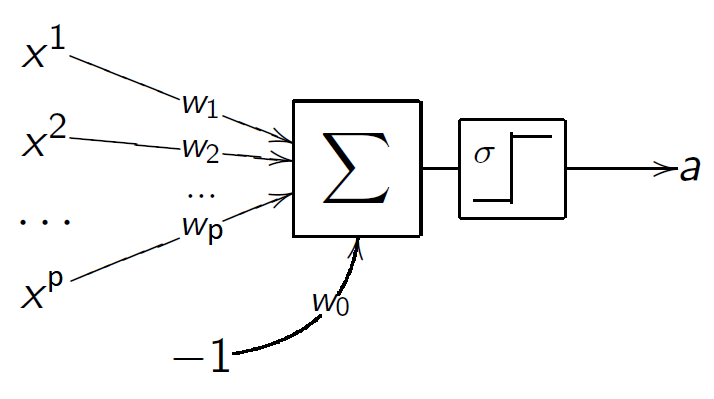
\includegraphics[scale=0.3]{mp2}
	\end{center}
     \column{.4\textwidth}
\begin{center}
	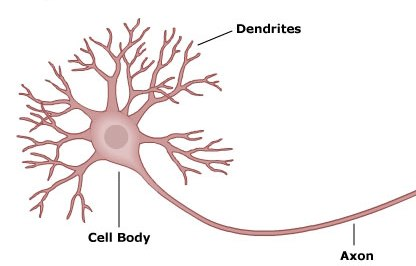
\includegraphics[scale=0.4]{neuron}
	\end{center}
\end{columns} 
\end{frame}


\begin{frame}
\frametitle{Способность аппроксимировать. Модель нейрона для задач машинного обучения}
%\textbf{Напоминание обозначений:} $X$ --- множество объектов, $Y$ --- множество ответов; $(f_1(x),\ldots,f_p(x))$ --- признаки объекта $x \in X$; $x^j:= f_j(x)$;\\$X^n = (x_i, y_i)_{j=1}^{n}$ --- обучающая выборка.\\
%\vspace{0.5cm}
%$(x_j, y_j)$ --- выборка, $x_j \in \mathbb{R}^p$, $y_j \in \mathbb{R}$, $j=1,\ldots,n$.\\
%\vspace{0.2cm}
\textbf{Задача регрессии}: $Y= \mathbb{R}$, $a(x_j,w) = \sigma( \langle w,x_j \rangle )$,

\begin{equation*}
Q(w; X^{n})=\sum_{j=1}^{n} \mathscr{L} \left( \langle w,x_j \rangle, y_j \right)=\sum_{j=1}^{n}\left( \sigma( \langle w,x_j \rangle ) -y_j \right)^2 \rightarrow \min_{w}.
\end{equation*}

При $\sigma(z) = z$ получаем многомерную линейную регрессию.\\
\vspace{0.9cm}
\textbf{Задача классификации}: $Y =\{ \pm 1 \}$, $a(x_j,w) = \sign \langle w,x_j \rangle$,

\begin{equation*}
Q(w; X^{n})=\sum_{j=1}^{n} \mathscr{L} \left( \langle w,x_j \rangle, y_j \right) = \sum_{j=1}^{n} [y_j \langle w,x_j \rangle  < 0] \rightarrow \min_{w}.
\end{equation*}\\
\vspace{0.9cm}
\textbf{Нейронная сеть} --- суперпозиция нейронов.\\
\textcolor{red}{Насколько богатый класс функций реализуется нейроном? А сетью?}
\end{frame} 
  
\begin{frame}
\frametitle{Способность аппроксимировать. Нейронная реализация логических функций}
\vspace{0.1cm}
Функции И, ИЛИ, НЕ от бинарных переменных $x^1$ и $x^2$:
\begin{gather*}
x^1 \wedge x^2 = \left[x^1 + x^2 - \frac{3}{2} > 0\right]; \\
x^1 \vee x^2 = \left[x^1 + x^2 - \frac{1}{2} > 0 \right]; \\
\neg x^1 = \left[-x^1 - \frac{1}{2} > 0 \right].
\end{gather*}
 
\begin{center}
	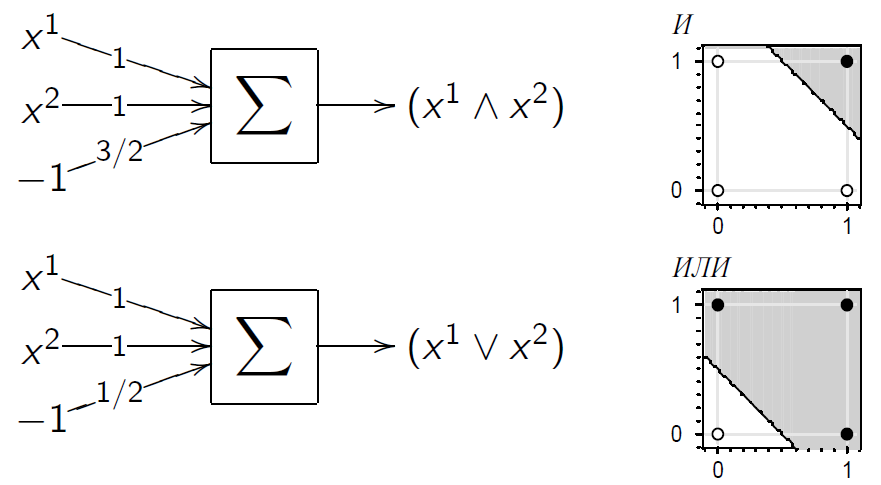
\includegraphics[scale=0.27]{and_or}
\end{center}
\end{frame}  

 
\begin{frame}
\frametitle{Способность аппроксимировать. Функция XOR}
\vspace{0.1cm}
$x^1 \oplus x^2 = [ x^1 \neq x^2]$ \textcolor{red}{не реализуема} одним нейроном. 2 варианта реализации:\\
\vspace{0.3cm}
1. добавление нелинейного признака:
\begin{gather*}
x^1 \oplus x^2 = \left[x^1 + x^2 - \textcolor{red}{2 x^1 x^2} - \frac{1}{2} > 0\right]; \\
\end{gather*}
2. двухслойной \textcolor{red}{нейронной сетью} (суперпозицией) функций И, ИЛИ, НЕ:
\begin{gather*}
x^1 \oplus x^2 = \left[ \neg \left( x^1 \wedge x^2 - x^1 \vee x^2 \right)  > 0\right]. \\
\end{gather*}

\begin{center}
	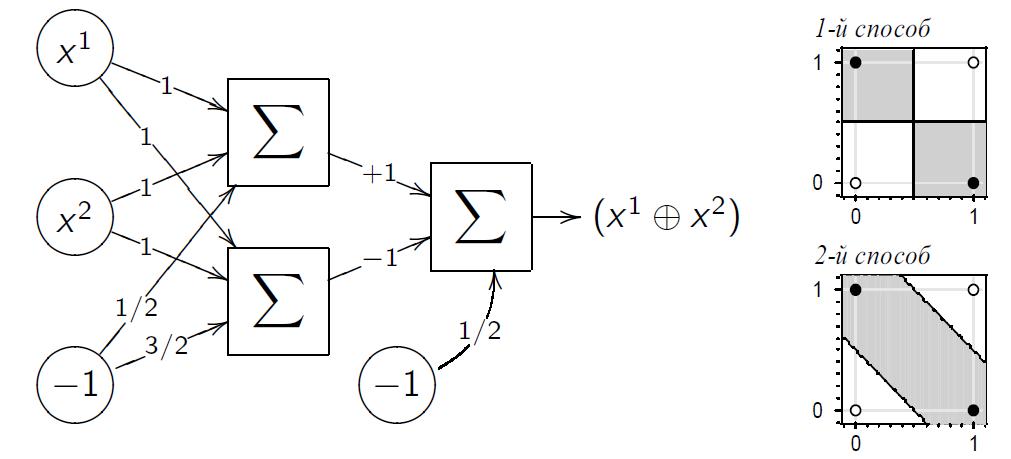
\includegraphics[scale=0.27]{xor}
\end{center}
\end{frame} 

\begin{frame}
\frametitle{Способность аппроксимировать. Можно ли любую функцию представить нейросетью?}

\begin{theorems}[Цыбенко, 1989]
Пусть $\sigma(x)$ --- непостоянная, ограниченная и монотонно возрастающая непрерывная функция;\\
$I_{p_0}$ --- ${p_0}$-мерный единичный гиперкуб;\\
$C(I_{p_0})$ --- множество непрерывных функций на $I_{p_0}$.\\
Тогда для любой $f \in C(I_{p_0})$ и $\varepsilon > 0$ существуют $p_1 \in \mathbb{Z}$ и  $\alpha_i$, $b_i$, $w_{ij} \in \mathbb{R}$, $i=1,\ldots,p_1$, $j=1,\ldots, p_0$, такие что функция
\begin{equation*}
F(x^1, \ldots, x^{p_0})=\sum_{i=1}^{p_1} \alpha_i \, \sigma \left(\sum_{j=1}^{p_0} w_{ij} x^j + b_i   \right),
\end{equation*}
аппроксимирует функцию $f$ с точностью $\varepsilon$:
 \begin{equation*}
| F(x^1, \ldots, x^{p_0}) - f(x^1, \ldots, x^{p_0})| < \varepsilon
\end{equation*} 
для любого $x=(x^1, \ldots, x^{p_0}) \in I_{p_0}$.
\end{theorems}

\end{frame} 

\begin{frame}
\frametitle{Способность аппроксимировать. Можно ли любую функцию представить нейросетью?}

\begin{equation*}
F(x^1, \ldots, x^{p_0})=\sum_{i=1}^{p_1} \alpha_i \, \sigma \left(\sum_{j=1}^{p_0} w_{ij} x^j + b_i   \right),
\end{equation*}
\\
\vspace{0.5cm} 
\textbf{Нейросеть, выход которой, соответствует F:}\\
сеть с $p_0$ входными узлами, одним скрытым слоем с $p_1$ узлами и функцией активации $\sigma(z)$. \\
\vspace{0.5cm} 

\textbf{Выводы:} 
\begin{itemize}
\item Любую непрерывную функцию можно приблизить нейросетью с любой заранее заданной точностью. 
\item Для этой нейросети нужна одна нелинейная функция активации и один скрытый слой.
\end{itemize}

\end{frame}


\begin{frame}
\frametitle{Расширяемость. Многослойная нейронная сеть}
Пусть для общности $Y = \mathbb{R}^M$ и слоёв для простоты только два.\\
\vspace{0.4cm} 
\begin{columns}
    \column{.3\textwidth}
   $\quad$ входной слой, \\
  $\quad$ $p$ признаков\\
  $\quad$ $\overbrace{\quad \quad \quad \quad \quad}$
     \column{.3\textwidth}
     скрытый слой, \\
     $H$ нейронов\\
   $\overbrace{\quad \quad \quad \quad \quad}$
     
      \column{.3\textwidth}
     $\,\,\,$ выходной слой, \\
     $\,\,\,$ $M$ нейронов\\
  $\,\,\,$  $\overbrace{\quad \quad \quad \quad \quad}$

\end{columns} 

\begin{center}
	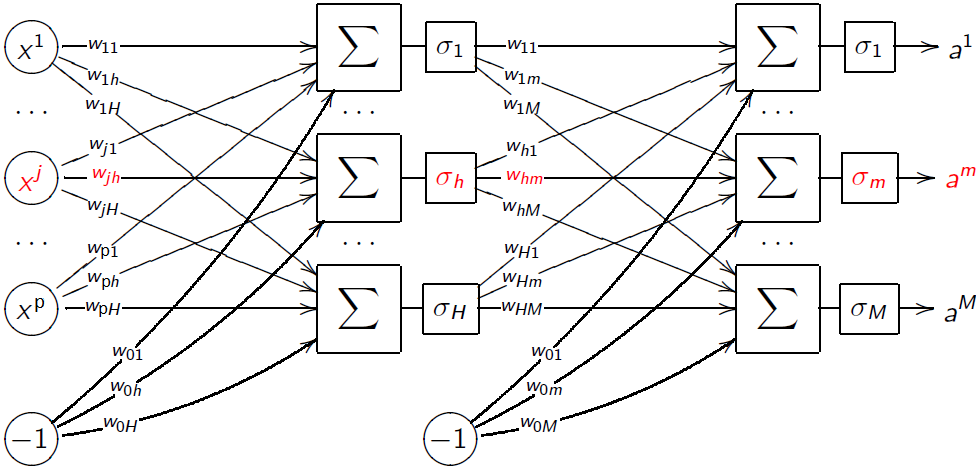
\includegraphics[scale=0.4]{nn2}
	\end{center} 	

Вектор параметров $w \equiv (w_{jh}, w_{hm}) = (\{ w_{jh}\}_{j,h=0}^{p,H}, \{w_{hm}\}_{h,m=0}^{H,M}) \in \mathbb{R}^{H(p+M+1) + M}$.
\end{frame}


\begin{frame}
\frametitle{Расширяемость. Многослойная нейронная сеть. \\Функция активации}
\vspace{0.4cm} 
\begin{itemize}
\item логистическая функция: $\sigma(z) = \frac{1}{1+e^{-a\,z}}$, $a \in \mathbb{R}$;
\item гиперболический тангенс: $\sigma(z) = \frac{e^{a\,z} - e^{-a\,z}}{e^{a\,z} + e^{-a\,z}}$, $a \in \mathbb{R}$;
\item rectifier: $f(z) = \max (0,x)\approx \ln (1 + e^z)$.
\end{itemize}

\begin{figure}
	\begin{center}
	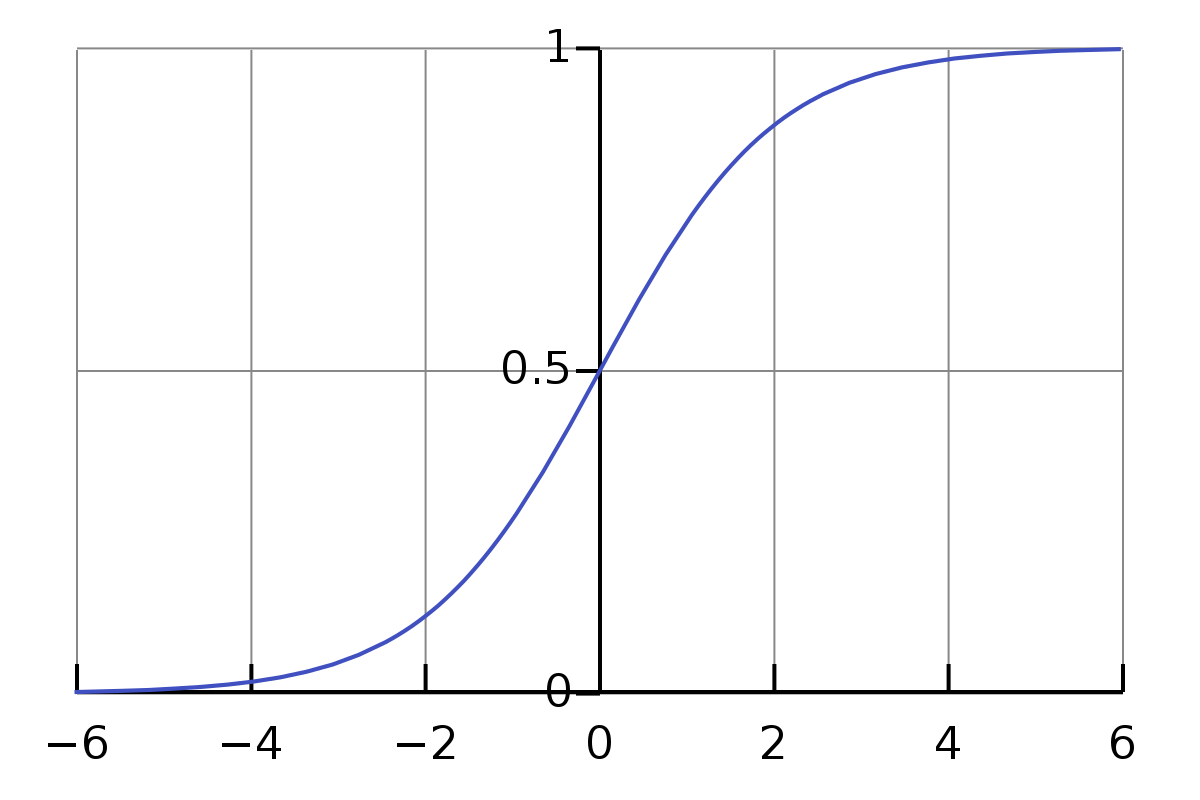
\includegraphics[scale=0.15]{Logistic_curve}
	\end{center}
	\caption{График функции $\frac{1}{1+e^{-z}}$.}
	\label{fig:tau}
\end{figure} 
\end{frame}


%\begin{frame}
%\frametitle{Backprop. Постановка задачи}
%Стандартная постановка задачи обучения с учителем.\\
%\vspace{1cm} 
%$X$ --- множество объектов, $Y$ --- множество ответов;\\
% $(f_1(x),\ldots,f_p(x))$ --- признаки объекта $x \in X$; $x^j:= f_j(x)$;\\$X^n = (x_i, y_i)_{j=1}^{n}$ --- обучающая выборка.\\
%\vspace{1cm} 
%Хотим построить отображение $X \rightarrow Y$ (нейросеть), которое минимизирует эмпирический риск:
%\begin{equation*}
%Q(w, X^n) = \frac{1}{n} \sum_{j=1}^{n} \mathscr{L}(w,x_i,y_i) \rightarrow \min_w.
%\end{equation*}
%\end{frame}

\begin{frame}
\frametitle{BackProp. Напоминание: алгоритм Stochastic Gradient}

Идея: на каждом шаге учитывать только одно наблюдение. \\
	\vspace{0.4cm} 
	Алгоритм: \\
	\vspace{0.2cm} 
	\begin{itemize}
		\item Инициализация вектора параметров $w^{(0)}$, выбор скорости обучения $\eta$, темп забывания $\lambda$, начальная оценка функционала 
		$$\overline{Q}(w_0)=\frac{1}{n} Q(w_0)=\frac{1}{n} \sum_{i=1}^n \mathscr{L}(w_0,x_i,y_i).$$
		\item Случайный выбор элемента из выборки $x_i$ и вычисление функции потерь $\mathscr{L}_i:=\mathscr{L}(w,x_i,y_i)$.
		\item Обновление вектора параметров $w:=w- \eta \textcolor{red}{\nabla \mathscr{L}(w,x_i,y_i)}$.
		\item Оценка функционала $Q :=(1-\lambda)Q+\lambda \mathscr{L}_i$.
		\item Повторять до сходимости $Q$ или $w$.
	\end{itemize}

\end{frame} 

\begin{frame}
\frametitle{BackProp. Дифференцирование суперпозиции функций}
Выходные значения сети $a^m(x_i)$, $m=1,\ldots,M$ на объекте $x_i$:
\begin{equation*}
 a^m(x_i) = \sigma_m \left(\sum_{h=0}^{H} w_{hm}  \textcolor{red}{ u^h(x_i)}  \right); \quad \quad \quad 
 \textcolor{red}{ u^h(x_i)} = \sigma_h \left(\sum_{j=0}^{p} w_{jh} f_j(x_{i})   \right).
\end{equation*} \\
	\vspace{0.4cm} 

Пусть для конкретности $\mathscr{L}_i(w)$ --- средний квадрат ошибки:
\begin{equation*}
\mathscr{L}_i(w) = \frac{1}{2} \sum_{m=1}^{M}(a^m(x_i) - y^m_i)^2.
\end{equation*}\\
	\vspace{0.4cm} 
\textbf{Промежуточная задача:} найти частые производные 
\begin{equation*}
 \frac{\partial \mathscr{L}_i(w)}{\partial a^m}; \quad \frac{\partial \mathscr{L}_i(w)}{\partial u^h}.
\end{equation*} \\
\end{frame} 

\begin{frame}
\frametitle{BackProp. Быстрое вычисление градиента}
\textbf{Промежуточная задача:} частая производная 
\begin{equation*}
 \frac{\partial \mathscr{L}_i(w)}{\partial a^m} = a^m(x_i) - y_i^m = \varepsilon_i^m
\end{equation*}
--- это ошибка на выходном слое.
\begin{equation*}
 \frac{\partial \mathscr{L}_i(w)}{\partial u^h} = \sum_{m=1}^{M}(a^m(x_i) - y_i^m) \sigma^{'}_m w_{hm} =\sum_{m=1}^{M} \varepsilon_i^m  \sigma^{'}_m w_{hm} =\varepsilon_i^h
\end{equation*}
--- назовём это \textit{ошибкой на скрытом слое}. \\
\vspace{0.4cm}
Похоже, что $\varepsilon_i^h$ вычисляется по $\varepsilon_i^m$, если запустить сеть <<задом наперёд>>:
  \begin{columns}
    \column{.4\textwidth}
   \begin{center}
	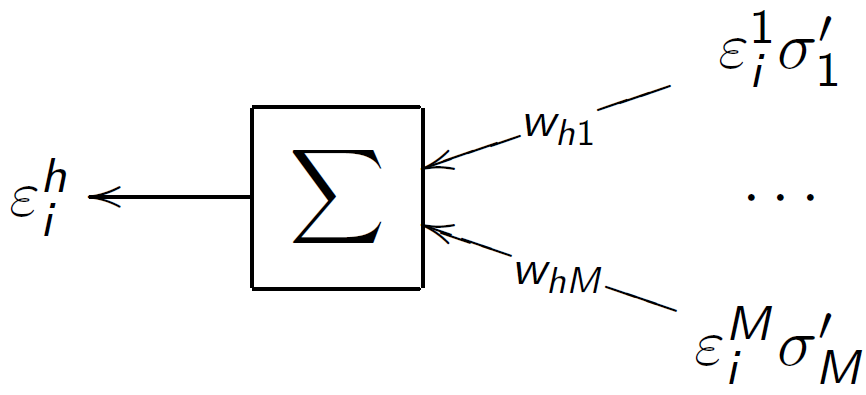
\includegraphics[scale=0.2]{backprop}
	\end{center}
     \column{.4\textwidth}
    
\end{columns} 
\end{frame} 

\begin{frame}
\frametitle{BackProp. Быстрое вычисление градиента}
Теперь, имея частные производные $\mathscr{L}_i(w)$ по $a^m$ и $u^h$, легко выписать градиент $\mathscr{L}_i(w)$ по весам $w$:
\\
\vspace{0.4cm} 
\begin{align*}
\frac{\partial \mathscr{L}_i(w)}{\partial w_{hm}} &= \frac{\partial \mathscr{L}_i(w)}{\partial a^m} \frac{\partial a^m}{\partial w_{hm}}=\varepsilon_i^m \sigma_m^{'} u^h(x_i), \quad h=0,\ldots,H, \quad  m=1,\ldots,M; \\
\frac{\partial \mathscr{L}_i(w)}{\partial w_{jh}} &= \frac{\partial \mathscr{L}_i(w)}{\partial u^h} \frac{\partial u^h}{\partial w_{jh}}=\varepsilon_i^h \sigma_h^{'} f_j(x_{i}), \quad j=0,\ldots,p, \quad h=1,\ldots,H.
\end{align*}
\\
\vspace{0.7cm} 
 Под $ \sigma^{'}_m$ всегда будет подразумеваться производная в точке $\sum_{h=0}^{H} w_{hm} u^h(x_i)$. Аналогично, под $\sigma^{'}_h$ всегда будет подразумеваться производная в точке $\sum_{j=0}^{p} w_{jh} f_j(x_{i})$.  
\end{frame} 

\begin{frame}
\frametitle{BackProp. Алгоритм}
\textcolor{blue}{\bfseries Вход:} $X^n = (x_i, y_i)_{i=1}^{n} \subset \mathbb{R}^p \times \mathbb{R}^M$; параметры $H$, $\lambda$, $\eta$.\\
\textcolor{blue}{\bfseries Выход:} веса $w_{jh}$, $w_{hm}$. \\
1:инициализировать веса $w_{jh}$, $w_{hm}$;\\
2:\textcolor{blue}{\bfseries повторять} \\
3:$\quad \quad$случайно выбрать элемент  $x_i$ из выборки $X^n$; \\
4:$\quad \quad$прямой ход:\\
 $\quad \quad \,\,$ $u_i^h := \sigma_h \left( \sum_{j=0}^{p} w_{jh} x^j_{i}\right), \,\, h=1,\ldots,H;$\\
 $\quad \quad \,\,$ $a_i^m := \sigma_m \left( \sum_{h=0}^{H} w_{hm} u_{i}^h \right), \,\, \varepsilon_i^m := a_i^m - y_{im}, \,\, m=1,\ldots,M;$\\
 $\quad \quad \,\,$ $ \mathscr{L}_i := \sum_{m=1}^{M}(\varepsilon_i^m)^2, \text{ вычисление производных } \sigma_m^{'}, \sigma_h^{'}$;\\
5:$\quad \quad$обратный ход:\\
 $\quad \quad \,\,$ $\varepsilon_i^h := \sum_{m=1}^M \varepsilon_i^m \sigma^{'} w_{hm}$, $h=1,\ldots,H$;\\
6:$\quad \quad$градиентный шаг:\\
 $\quad \quad \,\,$ $w_{hm} := w_{hm} - \eta \varepsilon_i^m \sigma^{'}_m u_i^h$, $h=0,\ldots,H$, $ m=1,\ldots,M$;\\ 
 $\quad \quad \,\,$ $w_{jh} := w_{jh} - \eta \varepsilon_i^h \sigma^{'}_h x^j_{i}$, $j=0,\ldots,p$, $ h=1,\ldots,H$;\\
7:$\quad \,\,\,$ $Q := (1-\lambda) Q + \lambda\mathscr{L}_i$;\\
8:\textcolor{blue}{\bfseries пока:} $Q$ не сойдется.
\end{frame} 
 
\begin{frame}
\frametitle{BackProp. Преимущества и недостатки}
\textbf{Преимущества:}
\begin{itemize}
\item быстрое вычисление градиента;
\item метод легко обобщается на любые $\sigma$, $\mathscr{L}$;
\item возможно динамическое (потокое) обучение;
\item на сверхбольших выборках не обязательно брать все $x_i$;
\item возможность распараллеливания.
\end{itemize}
\vspace{0.7cm} 
\textbf{Недостатки (есть все те же, что и у SG):}
\begin{itemize}
\item возможна медленная сходимость;
\item застревание в локальных минимумах;
\item проблема <<паралича>> сети (горизонтальные асимптоты $\sigma$); 
\item проблема переобучения;
\item сложно подбирать эвристики.
\end{itemize}
\end{frame} 
  
\begin{frame}
\frametitle{BackProp. Эвристики}
Применимы все те же эвристики, что и в обычном SG:
\begin{itemize}
\item инициализация весов;
\item порядок предъявления объектов;
\item оптимизация величины градиентного шага;
\item регуляризация (сокращение весов). 
\end{itemize} 
 \vspace{0.7cm}
 И появляются новые эвристики для улучшения сходимости, специфичные для нейросети.
%Но появляются новые проблемы:
%\begin{itemize}
%\item выбор функций активации в каждом нейроне;
%\item выбор числа слоёв и числа нейронов;
%\item выбор значимых связей.
%\end{itemize} 

\end{frame} 

\begin{frame}
\frametitle{Эвристики для нейросети. Начальное приближение}
 Более тщательный подбор начального приближения.\\
 \vspace{0.7cm}
Нейроны первого слоя настраиваются как $H$ отдельных однослойных сетей:
\begin{itemize}
\item либо по случайной подвыборке $X^{'} \subseteq X^n$;
\item либо по случайному подмножеству входов;
\item либо из различных случайных начальных приближений;
\end{itemize}
тем самым обеспечивается \textit{различность нейронов}.\\
 \vspace{0.9cm}
Затем по отдельности настраиваются нейроны второго слоя, которым на вход подается вектор выходных значений первого. 
\\
 \vspace{0.9cm}
 %По сути такая двухслойная сеть является простейшей алгоритмической композицией (bagging).
 
%2. Выбивание из локальных минимумов (jogging of weights).
%3. Адаптивный градиентный шаг (метод скорейшего спуска).
%4. 
\end{frame} 

\begin{frame}
\frametitle{Эвристики для нейросети. Выбор градиентного метода}
 1. \textbf{Адаптивный градиентный шаг} (метод скорейшего спуска). Ищем $\eta_*$:
 \begin{equation*}
  \mathscr{L}_i(w - \nabla \mathscr{L}_i(w)) \rightarrow \min_\eta.
 \end{equation*}
 2. \textbf{Диагональный метод Левенберга-Марквардта.}\\
   \vspace{0.2cm}
 Метод Ньютона-Рафсона (второго порядка):
 \begin{equation*}
 w := w - \eta (\mathscr{L}_i^{''}(w))^{-1} \mathscr{L}_i^{'}(w),
 \end{equation*}
 где $\mathscr{L}_i^{''}(w) = \left( \frac{\partial^2 \mathscr{L}_i(w) }{\partial w_{jh} \partial w_{j^{'}h^{'}}}   \right)$ --- гессиан размера $(H(p+M+1) + M)^2$.\\
  \vspace{0.4cm}
 \textbf{Эвристика.} Считаем, что гессиан диагонален:
 \begin{equation*}
 w_{jh} := w_{jh} - \eta \left(  \frac{\partial^2 \mathscr{L}_i(w) }{\partial w_{jh}^2} + \mu  \right) ^{-1} \frac{\partial \mathscr{L}_i(w) }{\partial w_{jh}}, 
\end{equation*}  
$\eta$ --- темп обучения, \\
$\mu$ --- параметр, предотвращающий обнуление элемента.
\end{frame} 

\begin{frame}
\frametitle{Построение нейросети}

\structure{Выбор числа скрытых слоёв.} Двух-трёх слоёв достаточно для очень широкого класса задач. Если знаем, что классы линейно разделимы, то достаточно одного слоя.\\ 
\vspace{1cm}
\structure{Выбор числа нейронов в скрытом слое H.} \\ 
\begin{itemize}
\item \textbf{Визуальный способ} (для задач с небольшим числом признаков). Если граница классов (или кривая регрессии) слишком сглажена --- размер слоя нужно увеличить, а если есть резкие колебания, то, наоборот, уменьшить.
\item \textbf{По внешнему критерию.} 
\begin{itemize}
\item Средняя ошибка на тестовой выборке. 
\item CV (главный недостаток --- высокая трудоёмкость).
\end{itemize}

\end{itemize}

\end{frame}


\begin{frame}
\frametitle{Построение нейросети. Динамическое наращивание сети}


\begin{enumerate}
\item Обучение при заведомо недостаточном числе нейронов $H \ll n$ до тех пор, пока ошибка не перестаёт убывать.
\item Добавление нового нейрона и инициализация его связей небольшими случайными весами или путем обучения 
\begin{itemize}
\item либо по случайной подвыборке $X^{'} \subseteq X^n$;
\item либо по объектам с наибольшими значениями потерь;
\item либо по случайному подмножеству входов;
\item либо из различных случайных начальных приближений.
\end{itemize}
Веса старых связей не меняются.
\item Снова итерации BrackPop.
\end{enumerate}
\vspace{0.6cm}
Полезно наблюдать за внешним критерием. Например, прохождение $Q(X^k)$ через минимум --- надежный критерий остановки. \\
  \vspace{0.6cm}
  \textbf{Эмпирический опыт:} Общее время обучения обычно лишь в $1.5$--$2$ раза больше, чем если бы в сети сразу было нужное количество нейронов. Полезная информация, накопленная сетью, не теряется при добавлении новых нейронов. 
\end{frame} 

\begin{frame}
\frametitle{Построение нейросети. Удаление избыточных связей. Optimal Brain Damage (OBD)}
Пусть $w$ --- локальный минимум $Q(w)$, \\тогда $Q(w)$ можно аппроксимировать квадратичной формой:
\begin{equation*}
Q(w + \delta) = Q(w) + \frac{1}{2} \delta^{\mathrm{T}} Q^{''}(w) \delta + o(\| \delta\|^2),
\end{equation*}
где $Q^{''}(w) =  \frac{\partial^2 Q(w) }{\partial w_{jh} \partial w_{j^{'}h^{'}}}$ --- гессиан размера $(H(p+M+1) + M)^2$.\\
 \vspace{0.6cm}
 \textbf{Эвристика.} Пусть гессиан диагонален, тогда
 \begin{equation*}
  \delta^{\mathrm{T}} Q^{''}(w) \delta = \sum_{j=0}^{p}\sum_{h=0}^{H} \delta^2_{jh}   \frac{\partial^2 Q(w) }{\partial w_{jh}^2 }  +  \sum_{h=0}^{H}\sum_{m=0}^{M} \delta^2_{hm}   \frac{\partial^2 Q(w) }{\partial w_{hm}^2 }.
 \end{equation*}
 Хотим обнулить вес: $w_{jh} + \delta_{jh}=0$. Как изменится $Q(w)$?\\
  \vspace{0.6cm}
  \textbf{Определение.} \textit{Значимость} веса $w_{jh}$ --- это изменение функционала $Q(w)$ при его обнулении: $S_{jh} = w^2_{jh}  \frac{\partial^2 Q(w) }{\partial w_{jh}^2 } $.
\end{frame} 

\begin{frame}
\frametitle{Построение нейросети. Удаление избыточных связей. Optimal Brain Damage (OBD)}
\begin{enumerate}
\item В BackProp вычислять вторые производные $\frac{\partial^2 Q(w) }{\partial w_{jh}^2 } $,  $\frac{\partial^2 Q(w) }{\partial w_{hm}^2 } $.
\item Если процесс минимизации $Q(w)$ пришел в минимум, то
\begin{itemize}
\item упорядочить веса по убыванию $S_{jh}$;
\item удалить $d$ связей с наименьшей значимостью;
\item снова запустить BackProp.
\end{itemize}
\item Если $Q(w, X^n)$ или $Q(w, X^k)$ существенно ухудшился, то вернуть последние удаленные связи и выйти.
\end{enumerate}
  \vspace{0.5cm}
Аналогично, OBD можно использовать для \textbf{отбора признаков}.\\
Суммарная значимость признака: $S_j = \sum_{h=1}^{H} S_{jh}$.\\
 \vspace{0.5cm}
 \textbf{Эмпирический опыт:} сеть, построенная с помощью OBD, меньше переобучается, чем сеть сразу построенная по полученной структуре (со случайно инициализированными весами).
\end{frame} 
   
\end{document}
